\documentclass{icnmmf5}
\selectlanguage{english}
\usepackage{natbib}
\bibliographystyle{abbrv}

% Your title goes here.
\title{Prediction of averaged inter particles' properties within a buoyant emulsion by the use of \textit{Nearest Particle Statistics}}

% The author list. A \thanks{} is used to give an email address.
% This is only required for the corresponding author.
\author{Fintzi Nicolas\thanks{Email:~nicolas.fintzi@ifpen.fr}\\IFP Energies Nouvelles\and
Pierson Jean-Lou\thanks{Email:~jean-lou.pierson@ifpen.fr}\\IFP Energies Nouvelles
\and
St\'ephane Popinet\thanks{Email:~popinet@basilisk.fr}\\Sorbonne Universite}

% Empty date for \maketitle. Don't modify.
\date{}

\begin{document}
\maketitle

The population balance and averaged Navier Stokes equations have been used in engineering for decades. 
However, there is a clear lack of accurate closure regarding the coalescence source term in emulsion modeling.  
Therefore, in a multiscale strategy we used the code Basilisk ({http://basilisk.fr}) to perform tri-periodic simulations of buoyant emulsions, see Figure \ref{fig:tower}~(left). 
In addition, to providing data for the closure terms appearing in the averaged models, tri-periodic simulations are of great interest to understand and describe pairwise interactions of rising droplets. 
Which is a first step to the modeling of the closure terms in the averaged models. 
%  crucial information, if we aim to model coalescence phenomenon based on film drainage analysis. 

Therefore, in this work, we present a statistical analysis of droplets interaction based on the recent \textit{Nearest Particle Statistics} framework of \cite{zhang2021ensemble}.
We define a pair by a particle and its nearest neighbor. 
% This enables us to describe, the relative or absolute, characteristics of droplets pair.
From this analysis we propose a qualitative description of : 
the averaged relative position, velocity and acceleration of colliding pairs (see Figure \ref{fig:tower}~(right)), and the averaged wake of a non-isolated particles (see Figure \ref{fig:tower}~(middle)).
From the observation of these statistics we are clearly able to identify phenomenons such as  drafting kissing thumbing mechanism, clustering and the different wakes' shapes produce by the droplets.   
We also provide quantitative results such as the closure for the particle-fuild-particle stress tensor, as it has been defined in \cite{zhang2021ensemble}. 
This tensor describes long range interactions between droplets, it has been shown to be crucial to ensure the hyperbolicity of the averaged NS equations \cite{fox2020hyperbolic}. 

Overall, we expose the results of a parametric analysis focusing on the influence of droplets volume fraction, surface tension and inertial behavior, on the microstructure kinematic and dynamic interactions.
This leads us to an intuitive understanding of the different regime of interactions present in a buoyant emulsion. 
\begin{figure}[b]
  \begin{center}
   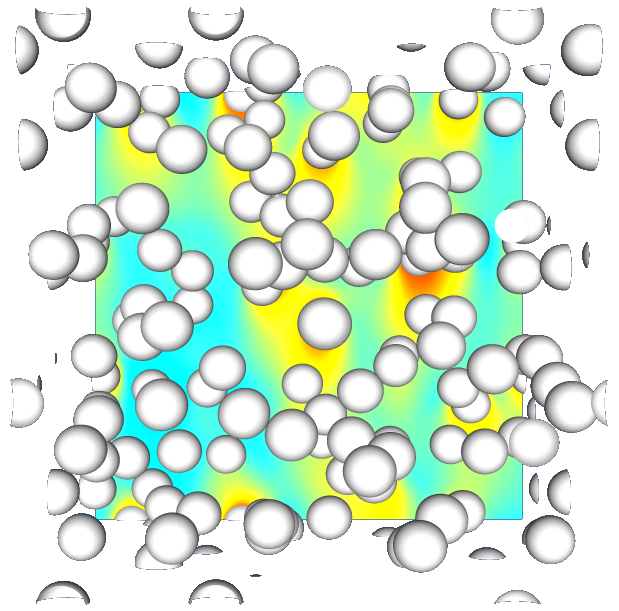
\includegraphics[height=4.5cm]{image/3D/P_PHI_5.png}
   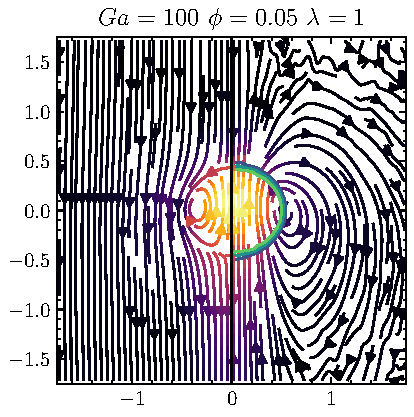
\includegraphics[height=4.5cm]{image/HOMOGENEOUS/Stream/Stream_PHI_5_Ga_100_l_1.pdf}
   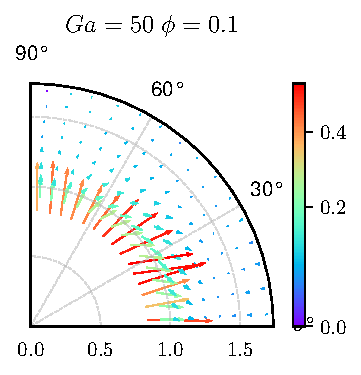
\includegraphics[height=4.5cm]{image/HOMOGENEOUS/fDrop/F_mu_r_1_0_Ga_50_PHI_0_1.pdf}
  \end{center}
  \caption{(left) DNS of a buoyant emulsion with finite size 125 droplets using volume of fluid method.
  (middle) Reconstruction of the nearest particle averaged eulerian velocity field.
  (right) Reconstruction of the nearest particle averaged center of mass acceleration field.}
  \label{fig:tower}
\end{figure}
\bibliography{Bib/bib_bulles.bib}
\end{document}
%%%%%%%%%%%%%%%%%%%%%%%%%%%%%%%%%%%%%%%%%%%%%%%%%%%%%%%%%%%%%%%%%%%%%%%%%%%%%%%%%%%%%%%%%%%%%%%%%%%%%%%
